% -*- root: ../thesis.tex -*-
%!TEX root = ../thesis.tex
% ******************************* Thesis Chapter 1 ****************************

% the code below specifies where the figures are stored
\ifpdf
    \graphicspath{{1_introduction/figures/PNG/}{1_introduction/figures/PDF/}{1_introduction/figures/}}
\else
    \graphicspath{{1_introduction/figures/EPS/}{1_introduction/figures/}}
\fi
% ----------------------------------------------------------------------
%: ----------------------- introduction content ----------------------- 
% ----------------------------------------------------------------------



%: ----------------------- HELP: latex document organisation
% the commands below help you to subdivide and organise your thesis
%    \chapter{}       = level 1, top level
%    \section{}       = level 2
%    \subsection{}    = level 3
%    \subsubsection{} = level 4
% note that everything after the percentage sign is hidden from output



\section{Background:} % section headings are printed smaller than chapter names
% intro
 The cloud hype has reached the Enterprise. It is expected that the Web 3.0 the Internet of things and data will revolve around the B-B market needs. For the latter, cloud implies the industrialization of delivery of managed services this means “employing a new consumption model inspired by the consumer internet services (B-C). 

Corporations have started to embrace and some have already adopted the 'cloud' delivery model of managed services. Very much like the SOA approach, 

One key area that must be looked at are the outdated, very often inflexible and slow resource allocation processes. Over the years these homegrown IT-Processes have become a major show stopper when it comes to a more dynamic and flexible resource allocation. The established deployment processes no longer satisfy demand in an ‘Everything as a Service’ (EaaS) world. The way out of this dilemma is the adoption of ‘Cloud’-technology. The latter has industrialized the delivery of managed services by employing a new consumption model and thus showing a clear way out into a more efficient IT-Infrastructure.

For example a multi-national bank, with its many different business models and related complex business scenarios that require elaborated workflows. Such a bank has legacy data bases, data warehouses and Enterprise content management systems to support their business units with all the processing of business data created and associated digital information collected. Independent of business model employed an Enterprise is obliged to comply with corporate and legal compliance and therefore is forced to implement a governance model for all information it is responsible for. Enterprises need to know what information they have, who is authorized to access it, how long the information needs to be kept and when it must be disposed. 

These four fundamental business characteristics imply that a catalog record must always point to its data counterpart, data can’t be orphaned nor should there be unknown duplicates. Companies already use an infrastructure to support their business processes and also satisfy their business intelligence needs using data bases, data marts, content management systems and a heterogeneous, geographically distributed repository landscape. What has been missing in the past were new tools to better handle the sheer volumes of data and scale in processing power required.   
 
We believe that the Cloud hype has brought fresh wind, new technologies and methods to boost Analytics and Discovery together with the promise to help cope the sheer volumes of information, the scale of processing power required and the benefit of flexible and cost-effective common infrastructure. We would like to show that Enterprise Content Management Systems and the ‘Cloud’ complement each other well to the benefit of every business that requires both content management and large scale analytics.




\subsection{Goals} % subsection headings are again smaller than section names
% lead
With this master thesis we want to investigate how the architecture design of legacy ECM Systems can be evolved such for being able to exploit todays cloud technologies in a non-disruptive way and thus overcoming current issues.  We believe the benefits for ECM from embracing the 'Cloud': the exploitation of the economies-of-scale, an inherent support for multi-tenancy, and the ubiquity of the service offering in an increasingly secure and trusted environment. \footnote{Enterprise Content Management - ECM}.  

\subsection{Expectations} % subsection headings 
Focus of this master thesis is to analyze the legacy architecture of ECM Systems, describe the shortcomings of the current design component by component and then develop a strategy to change, enhance and evolve the design in a way that allows the integration with current and future 'cloud technology’ in a non-disruptive way.

%: ----------------------- HELP: special characters
% above you can see how special characters are coded; e.g. $\alpha$
% below are the most frequently used codes:
%$\alpha$  $\beta$  $\gamma$  $\delta$

%$^{chars to be superscripted}$  OR $^x$ (for a single character)
%$_{chars to be suberscripted}$  OR $_x$

%>  $>$  greater,  <  $<$  less
%≥  $\ge$  greater than or equal, ≤  $\ge$  lesser than or equal
%~  $\sim$  similar to

%$^{\circ}$C   ° as in degree C
%±  \pm     plus/minus sign

%$\AA$     produces  Å (Angstrom)

%: ----------------------- HELP: references
% References can be links to figures, tables, sections, or references.
% For figures, tables, and text you define the target of the link with \label{XYZ}. Then you call cross-link with the command \ref{XYZ}, as above
% Citations are bound in a very similar way with \cite{XYZ}. You store your references in a BibTex file with a programme like BibDesk.

\begin{figure}[htb]
  \centering
  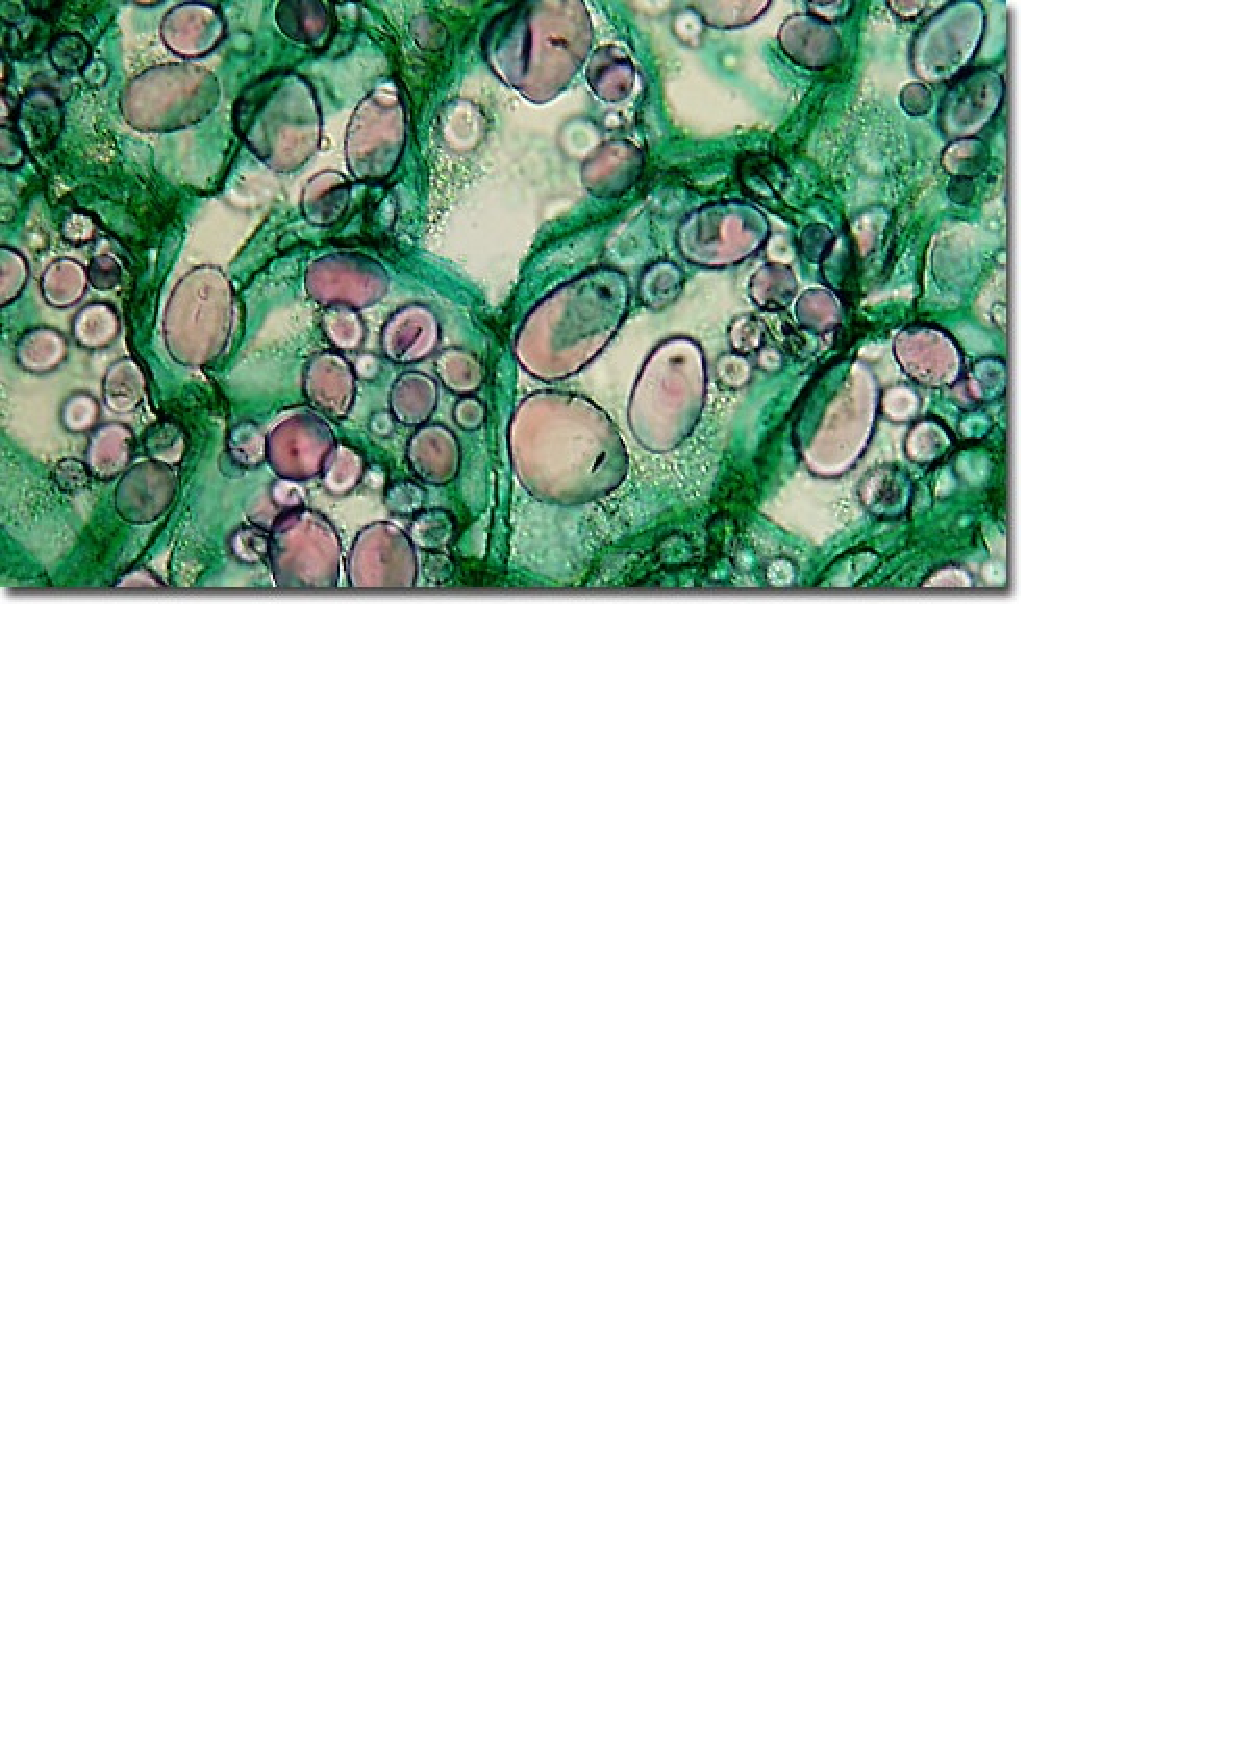
\includegraphics[width=1\columnwidth]{largepotato}
  \caption[Place your ECM picture here ]{\textbf{A common ECM system architecture design} - The figure 
  \href{http://molecularexpressions.com/micro/gallery/burgersnfries/burgersnfries4.html}{Molecular Expressions}.}
  \label{fig:largepotato}
\end{figure}

The work should first analyze the current system architecture then introduce design aspects of dynamic deployment and automated operations and finally demonstrate the feasibility that legacy ECM systems can take advantage of cloud technology like: 

\begin{itemize}
\item Continuous delivery \& Integration
\item Virtualization, and Containerization 
\item Automated Administration \& Operations 
\item Cloud enabled Monitoring \& Metering 
\item 
\end{itemize}

In the second more practical part of this master work, a prototype ECM service should be developed, implemented and deployed into a cloud environment. As result a qualitative and quantitative evidence is to be shown of the optimized efficiency and minimize resource consumption compared to its legacy counterpart.


%: ----------------------- HELP: lists
% This is how you generate lists in LaTeX.
% If you replace {itemize} by {enumerate} you get a numbered list.


 


%: ----------------------- HELP: tables
% Directly coding tables in latex is tiresome. See below.
% I would recommend using a converter macro that allows you to make the table in Excel and convert them into latex code which you can then paste into your doc.
% This is the link: http://www.softpedia.com/get/Office-tools/Other-Office-Tools/Excel2Latex.shtml
% It's a Excel template file containing a macro for the conversion.

\subsection{Approach} % subsection headings 

The detailed tasks are:
\begin{itemize}
\item Part I 
\begin{itemize}
\item Familiarize yourself with the current ECM system architecture design and its context
\item Perform a gap analysis relative to the new business requirements 
\item Document the design problems derived and think possible solutions.       
\item Research and classify current and future cloud technology. 
This means you should analyze and compare the different cloud technologies and / or products available on the market, company laboratories and research institutions. Here are examples of cloud products /technology: 
Openstack, IBM Red Hat / Openshift, Podman / Kubernetes, Puppet, AWS CloudFormation, Ansible, Chef, Terraform, Google Cloud Deployment Manager, Microsoft Azure Automation, Foreman, VMware vCenter Configuration Manager (VCM), Cisco Intelligent Automation for Cloud
\item Create a list of all possible candidates document their cloud technology and their key capabilities, detail the pro and cons. 	  
\item Using all the above, sketch out the design changes required to satisfy function and non-functional requirements
\item Create a concept design of  the new and revised system architecture, outline the operational extensions required for being able to integrate with the cloud environment(s) chosen
\item Consolidate the documentation so far and present your intermediate results
    \end{itemize}
\item Part II 
    \begin{itemize}
    \item Implement the prototype ECM service chosen
    \item Verify and validate that deployment topology works as expected
    \item Consider the integration points challenges and benefits
    \item Monitor consumption and the operations of new IT-Infrastructure. 
    Measure the efficiency and consumption figures and estimate the benefits
    gained with the new approach. 
    \item Consolidate the documentation so far and present your intermediate results
    \end{itemize}
\item Part III 
\begin{itemize}
    \item Evaluate the results and consolidate documentation so far  
    \item Explain the new 'cloud' delivery model', the enhanced service offering and the benefits to the own business units inside the company and customers outside.   
    \item Final presentation and explanation if the final results
    \end{itemize}
\end{itemize}



% There you go. You already know the most important things.


% ----------------------------------------------------------------------

\section{SI-Units}

Please use siunitx-package:
\SI{1}{\volt} = \SI{1}{\ohm} \SI{1}{\ampere}


